\documentclass[border=10pt]{standalone}

\usepackage{tikz}
\usepackage{tikzsymbols}
\usetikzlibrary{calc,patterns,shapes.geometric}

\def\centerarc[#1](#2)(#3:#4:#5){\draw[#1] ($(#2)+({#5*cos(#3)},{#5*sin(#3)})$) arc (#3:#4:#5);}

\begin{document}
	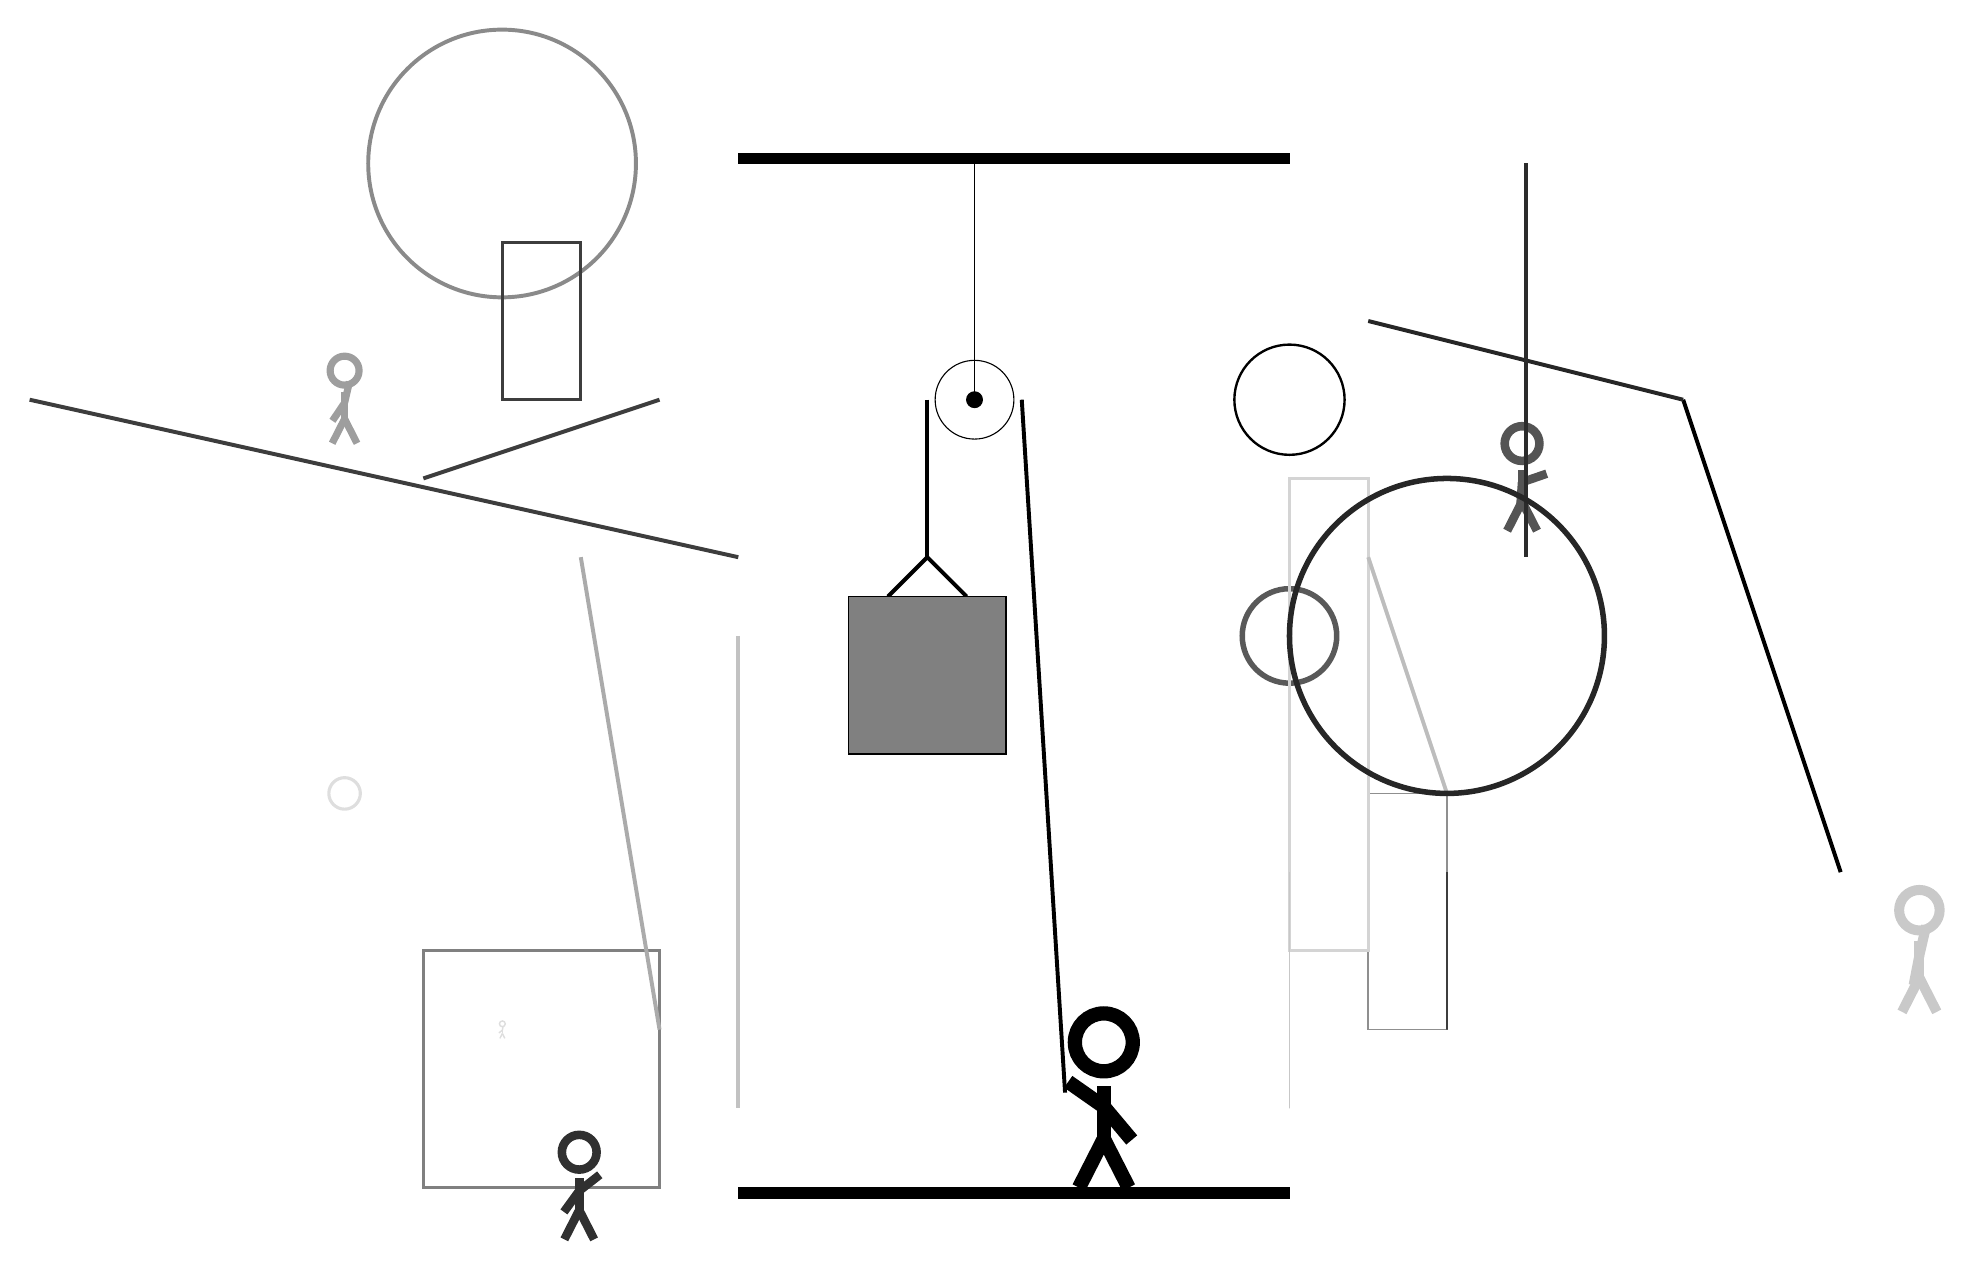
\begin{tikzpicture}
		%%%%% START %%%%%
		
		\draw[fill=black] (-2, 10) rectangle (5, 10.125);
		
		\draw (1, 7) circle (0.5);
		\draw[fill=black] (1, 7) circle (0.1);
		\draw (1, 10) -- (1, 7);
		
		\draw[line width=0.5mm] (-0.1, 4.5) -- (0.4, 5.0) -- (0.9, 4.5);
		\draw[fill=black!50] (-0.6, 4.5) rectangle (1.4, 2.5);
		
		\draw[line width=0.5mm] (0.4, 7) -- (0.4, 5.0);
		\centerarc[line width=0.5mm](1, 7)(0:180:0.6);
		\draw[line width=0.5mm](1.6, 7) -- (2.15, -1.8);
		
		\node at (2.6, -1.9) {\Strichmaxerl[10][-35][-50]};
		
		\draw[line width=0.5mm, color=black!100](10, 7) -- (12, 1);
		
		\draw [line width=0.5mm, color=black!46](-5, 10) circle (1.7);
		\node[line width=0.2mm, color=black!21] at (13, 0) {\Strichmaxerl[7][79][77]};
		\draw [line width=0.3mm, color=black!100](5, 7) circle (0.7);
		\draw[line width=0.5mm, color=black!24](-2, 4) -- (-2, -2);
		\draw[line width=0.2mm, color=black!44] (7, 2) rectangle (6, -1);
		\draw[line width=0.3mm, color=black!41] (-4, 7) rectangle (-4, 8);
		\draw[line width=0.4mm, color=black!76] (-4, 7) rectangle (-5, 9);
		\draw [line width=0.7mm, color=black!65](5, 4) circle (0.6);
		
		\draw[line width=0.5mm, color=black!76](-6, 6) -- (-3, 7);
		\draw[line width=0.5mm, color=black!85](10, 7) -- (6, 8);
		\node[line width=0.5mm, color=black!67] at (8, 6) {\Strichmaxerl[6][86][19]};
		\draw[line width=0.5mm, color=black!76](-2, 5) -- (-11, 7);
		\draw[line width=0.4mm, color=black!50] (-3, 0) rectangle (-6, -3);
		\node[line width=0.6mm, color=black!81] at (-4, -3) {\Strichmaxerl[6][54][38]};
		\node[line width=0.7mm, color=black!38] at (-7, 7) {\Strichmaxerl[5][56][77]};
		\draw[line width=0.4mm, color=black!17] (6, 6) rectangle (5, 0);
		\draw [line width=0.4mm, color=black!13](-7, 2) circle (0.2);
		\draw[line width=0.5mm, color=black!83](8, 10) -- (8, 5);
		\draw[line width=0.2mm, color=black!22] (5, -2) rectangle (5, 1);
		\node[line width=0.6mm, color=black!13] at (-5, -1) {\Strichmaxerl[1][37][79]};
		
		\draw[line width=0.5mm, color=black!33](-3, -1) -- (-4, 5);
		\draw[line width=0.5mm, color=black!26](7, 2) -- (6, 5);
		\draw[line width=0.3mm, color=black!76] (7, 1) rectangle (7, -1);
		\draw [line width=0.7mm, color=black!85](7, 4) circle (2.0);
		
		
		\draw[fill=black] (-2, -3) rectangle (5, -3.15);
		
		%%%%% END %%%%%
	\end{tikzpicture}
\end{document}